
\documentclass[12pt,aspectratio=169]{beamer}
\usepackage{amsmath, amssymb}
\usepackage{booktabs}
\usepackage{tikz}
\usetikzlibrary{arrows.meta,decorations.pathmorphing,patterns,calc,shadings}
\usepackage{xcolor}
\usepackage{array}

% -- Theme (identical to all previous decks) ---------------------------
\usetheme{Madrid}
\definecolor{firered}{RGB}{180,30,10}
\definecolor{ashgrey}{RGB}{50,55,65}
\definecolor{skyblue}{RGB}{30,100,180}
\definecolor{flameyellow}{RGB}{230,155,15}
\setbeamercolor{palette primary}{bg=ashgrey,fg=white}
\setbeamercolor{palette secondary}{bg=ashgrey!85,fg=white}
\setbeamercolor{palette tertiary}{bg=ashgrey!65,fg=white}
\setbeamercolor{palette quaternary}{bg=ashgrey,fg=white}
\setbeamercolor{structure}{fg=skyblue}
\setbeamercolor{alerted text}{fg=firered}
\setbeamercolor{block title}{bg=skyblue,fg=white}
\setbeamercolor{block body}{bg=skyblue!8}
\setbeamercolor{block title alerted}{bg=firered,fg=white}
\setbeamercolor{block body alerted}{bg=firered!10}
\setbeamercolor{block title example}{bg=ashgrey,fg=white}
\setbeamercolor{block body example}{bg=ashgrey!10}
\setbeamerfont{title}{size=\Large,series=\bfseries}
\setbeamertemplate{navigation symbols}{}
\setlength{\itemsep}{1pt}

% -- Macros ------------------------------------------------------------
\newcommand{\Da}{\mathrm{Da}}
\newcommand{\Le}{\mathrm{Le}}
\newcommand{\Rey}{\mathrm{Re}}
\newcommand{\Sh}{\mathrm{Sh}}
\newcommand{\Nu}{\mathrm{Nu}}
\newcommand{\Sc}{\mathrm{Sc}}
% \Pr already defined by LaTeX
\newcommand{\wdot}{\dot{\omega}}
\newcommand{\mdot}{\dot{m}}
\newcommand{\Tad}{T_{\text{ad}}}
\newcommand{\Ts}{T_s}
\newcommand{\Tinf}{T_\infty}
\newcommand{\Yfs}{Y_{F,s}}
\newcommand{\Yfinf}{Y_{F,\infty}}
\newcommand{\rs}{r_s}
\newcommand{\rf}{r_f}
\newcommand{\Ds}{D_s}
\newcommand{\BM}{B_M}
\newcommand{\BT}{B_T}
\newcommand{\Bc}{B_c}
\newcommand{\Zst}{Z_{\text{st}}}
\newcommand{\tchem}{t_{\text{chem}}}
\newcommand{\Kd}{K}
\newcommand{\Kc}{K_c}
\newcommand{\td}{t_d}
\newcommand{\code}[1]{\texttt{#1}}

% =====================================================================
\title{Droplet Evaporation and Combustion}
\subtitle{The D$^2$ Law, Transfer Numbers, and Single Droplet Burning}
\author{Prof.Dr. Onur Tuncer}
\institute{ITU Dept. of Aeronautical Eng.}
\date{\today}

\begin{document}

\begin{frame}
  \titlepage
\end{frame}

\begin{frame}{Lecture Outline}
  \tableofcontents
\end{frame}

% =====================================================================
\section{Why Droplet Combustion Matters?}
% =====================================================================

\begin{frame}{Liquid Fuel in Aero-Propulsion}

  Almost all practical aero-engines burn \textbf{liquid fuel}:
  Jet-A, kerosene, liquid hydrogen, liquid methane, and rocket
  propellants.
  Combustion cannot begin until the fuel is vaporized.

  \begin{center}
  \renewcommand{\arraystretch}{1.35}
  \begin{tabular}{>{\bfseries}p{2.8cm} p{4.3cm} p{4.5cm}}
    \toprule
    System & Injection & Droplet physics \\
    \midrule
    Gas turbine & Pressure-swirl atomizer, air-blast
      & $d_0 \sim 30$--$80\,\mu$m; evaporation in
        primary zone ($\sim$3--8 ms) \\
    Afterburner & V-gutter wake injection
      & $d_0 \sim 100$--$300\,\mu$m; must evaporate
        \& burn in $< 3$ ms \\
    Liquid rocket & Coaxial / impinging injectors
      & $d_0 \sim 50$--$200\,\mu$m; $p = 100$--$200$ bar;
        diffusion-flame combustion \\
    Ramjet & Strut injection into supersonic flow
      & Very short residence time; $d_0 < 50\,\mu$m essential \\
    \bottomrule
  \end{tabular}
  \end{center}

  \begin{exampleblock}{Unit context}
    Units 4--7 treated gases.
    This unit adds the \textbf{liquid phase}: evaporation,
    vaporization kinetics, and single-droplet combustion.
    Spray combustion is the superposition of many droplet histories.
  \end{exampleblock}
\end{frame}

% =====================================================================
\section{The D\texorpdfstring{$^2$}{2} Evaporation Law}
% =====================================================================

\begin{frame}{Assumptions of the D$^2$ Law}

  The D$^2$ law is the simplest quantitative model of droplet
  evaporation.  It rests on four key assumptions:

  \begin{enumerate}
    \item \textbf{Spherical symmetry}: the droplet is a perfect
          sphere; flow is purely radial.
    \item \textbf{Quasi-steady evaporation}: the droplet radius
          changes slowly compared to diffusion timescales
          ($\rs^2/\alpha \ll t_d$).
    \item \textbf{Single-component liquid}: uniform composition and
          uniform surface temperature $\Ts$.
    \item \textbf{Constant properties}: $\rho D$, $\lambda$, $c_p$
          evaluated at a reference ``film'' temperature and
          treated as constant.
  \end{enumerate}

  \begin{block}{Coordinate system}
    Droplet radius $\rs(t)$; radial coordinate $r \geq \rs$.
    At $r = \rs$: liquid surface (boundary conditions).
    As $r \to \infty$: ambient conditions
    ($T = \Tinf$, $Y_F = \Yfinf$).
  \end{block}
\end{frame}

\begin{frame}{Deriving the Mass Evaporation Rate}

  In steady spherical flow, mass conservation gives:
  \[
    \mdot = 4\pi r^2 \rho v = \text{const}
    \qquad (v > 0 \text{ outward})
  \]
  The fuel vapour transport equation (convection + diffusion):
  \[
    \mdot\,\frac{dY_F}{dr}
    = 4\pi r^2 \rho D \frac{dY_F}{dr}
    \quad\Rightarrow\quad
    \frac{d}{dr}\!\left(r^2\rho D\frac{dY_F}{dr}\right)
    = \frac{\mdot}{4\pi}\frac{dY_F}{dr}
  \]
  Integrating with boundary conditions $Y_F(\rs) = \Yfs$,
  $Y_F(\infty) = \Yfinf$:
  \[
    \boxed{
      \mdot = 4\pi\rs\,\rho D\,\ln(1 + \BM)
    }
  \]
  where the \alert{Spalding mass transfer number} is:
  \[
    \BM = \frac{\Yfs - \Yfinf}{1 - \Yfs}
  \]
\end{frame}

\begin{frame}{The D$^2$ Law}

  The droplet mass is $m = \tfrac{4}{3}\pi\rs^3\rho_\ell$.
  Its rate of change equals the evaporation rate:
  \[
    \frac{dm}{dt} = 4\pi\rs^2\rho_\ell\frac{d\rs}{dt} = -\mdot
  \]
  Substituting $\mdot = 4\pi\rs\,\rho D\ln(1+\BM)$:
  \[
    \frac{d(\rs^2)}{dt} = -\frac{2\rho D}{\rho_\ell}\ln(1+\BM)
    \equiv -\Kd
  \]

  \begin{block}{The D$^2$ Law}
    \[
      \boxed{D^2(t) = D_0^2 - \Kd\,t}
      \qquad
      \Kd = \frac{8\rho D}{\rho_\ell}\ln(1+\BM)
      \quad [\text{m}^2/\text{s}]
    \]
    The square of the droplet \emph{diameter} decreases
    \textbf{linearly} with time.
    The droplet lifetime is:
    \[
      \td = \frac{D_0^2}{\Kd}
    \]
  \end{block}
\end{frame}

\begin{frame}{The D$^2$ Law: Graphical Representation}

  \begin{columns}
    \begin{column}{0.52\textwidth}
      \centering
      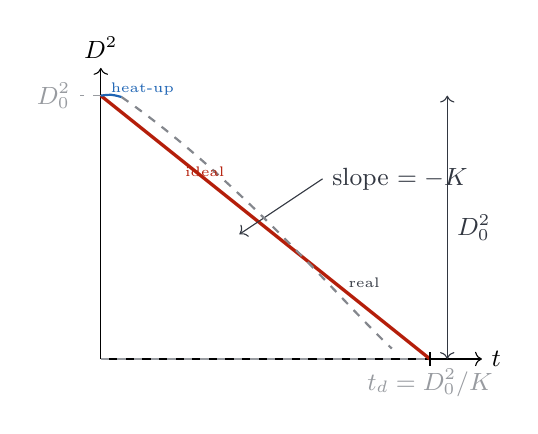
\begin{tikzpicture}[scale=0.88]
        % Axes
        \draw[->] (0,0) -- (5.5,0)
          node[right,font=\small]{$t$};
        \draw[->] (0,0) -- (0,4.2)
          node[above,font=\small]{$D^2$};
        % D^2 line (slope = -K)
        \draw[firered,very thick] (0,3.8) -- (4.75,0);
        % Annotations
        \draw[dashed,ashgrey!50] (0,3.8) -- (-0.3,3.8)
          node[left,font=\small]{$D_0^2$};
        \draw[<->,ashgrey,thin] (5.0,0) -- (5.0,3.8)
          node[midway,right,font=\small]{$D_0^2$};
        % Slope annotation
        \draw[<-,ashgrey,thin] (2.0,1.8) -- (3.2,2.6)
          node[right,font=\small]{slope $= -K$};
        % t_d annotation
        \draw[dashed,ashgrey!50] (4.75,0)
          node[below,font=\small]{$t_d = D_0^2/K$} -- (4.75,0.0);
        \draw[dashed,ashgrey!50,thin] (0,0) -- (4.75,0);
        % Tick
        \draw (4.75,-0.1)--(4.75,0.1);
        % Heating period (small initial transient)
        \draw[skyblue,thick]
          (0,3.8) .. controls (0.15,3.82) .. (0.3,3.78)
          -- (0.3,3.78);
        \node[skyblue,font=\tiny] at (0.6,3.9)
          {heat-up};
        % Real droplet deviation (dashed)
        \draw[ashgrey!60,dashed,thick]
          (0.3,3.78) .. controls (2.0,2.6) and (3.5,0.8) ..
          (4.2,0.15);
        \node[ashgrey,font=\tiny] at (3.8,1.1)
          {real};
        \node[firered,font=\tiny] at (1.5,2.7)
          {ideal};
      \end{tikzpicture}
    \end{column}
    \begin{column}{0.44\textwidth}
      \begin{itemize}
        \item $D^2$ decreases \textbf{linearly} in the ideal D$^2$
              law (straight red line)
        \item Short initial \textbf{heat-up period} while $\Ts$
              rises to the wet-bulb temperature
        \item Real droplets (dashed) deviate due to:
          \begin{itemize}
            \item Internal circulation
            \item Variable properties
            \item Forced convection
            \item Multi-component fuel
          \end{itemize}
        \item Despite simplifications, D$^2$ law captures
              $\td \propto D_0^2$ correctly
      \end{itemize}
    \end{column}
  \end{columns}
\end{frame}

\begin{frame}{The Spalding Transfer Number $\BM$}

  \[
    \BM = \frac{\Yfs - \Yfinf}{1 - \Yfs}
  \]

  \begin{columns}[t]
    \begin{column}{0.50\textwidth}
      \textbf{Surface fuel mass fraction $\Yfs$}\\[4pt]
      At the liquid surface, vapour--liquid equilibrium gives:
      \[
        \Yfs = \frac{W_F\,p_{\text{sat}}(\Ts)}
                    {W_F p_{\text{sat}} + W_{\text{air}}(p - p_{\text{sat}})}
      \]
      $p_{\text{sat}}(\Ts)$ is the Clausius--Clapeyron
      saturation pressure.
      Higher $\Ts$ $\Rightarrow$ higher $\Yfs$
      $\Rightarrow$ higher $\BM$ $\Rightarrow$ faster evaporation.
    \end{column}
    \begin{column}{0.46\textwidth}
      \textbf{Typical values (Jet-A, 1 atm)}
      \begin{center}
      \renewcommand{\arraystretch}{1.3}
      \begin{tabular}{lcc}
        \toprule
        $\Ts$ (K) & $\Yfs$ & $\BM$ \\
        \midrule
        350 & 0.10 & 0.11 \\
        400 & 0.28 & 0.39 \\
        450 & 0.55 & 1.22 \\
        500 & 0.82 & 4.56 \\
        \bottomrule
      \end{tabular}
      \end{center}
      \small $\BM \gg 1$: rapid evaporation (droplet near boiling).\\
      $\BM \ll 1$: slow evaporation (cold droplet).
    \end{column}
  \end{columns}
\end{frame}

\begin{frame}{Energy Balance: Wet-Bulb Temperature}

  The \textbf{wet-bulb temperature} $\Ts^*$ is the steady-state
  surface temperature at which the rate of heat conducted to the
  surface exactly supplies the latent heat of vaporisation.

  \medskip
  Energy balance at the droplet surface:
  \[
    \underbrace{\mdot\,L_v}_{\text{latent heat}}
    = \underbrace{4\pi\rs\,\lambda\ln(1+\BT)}_{\text{heat from gas}}
  \]
  where the \alert{thermal transfer number} is:
  \[
    \BT = \frac{c_p(\Tinf - \Ts)}{L_v + Q_{\text{sens}}}
    \approx \frac{c_p(\Tinf - \Ts)}{L_v}
  \]

  \begin{block}{Consistency condition}
    At steady state, $\BM = \BT$ (both transfer numbers must be equal
    for simultaneous heat and mass transfer).
    This determines the unique wet-bulb temperature $\Ts^*$.
    In practice, $\Ts^*$ is slightly below the boiling point at
    the local partial pressure of the vapour.
  \end{block}
\end{frame}

% =====================================================================
\section{Single Droplet Combustion}
% =====================================================================

\begin{frame}{Burning Droplet: Physical Picture}

  When the fuel vapour concentration around an evaporating droplet
  exceeds the rich flammability limit, a \textbf{spherical diffusion
  flame} forms at the stoichiometric surface.

  \begin{columns}
    \begin{column}{0.44\textwidth}
      \centering
      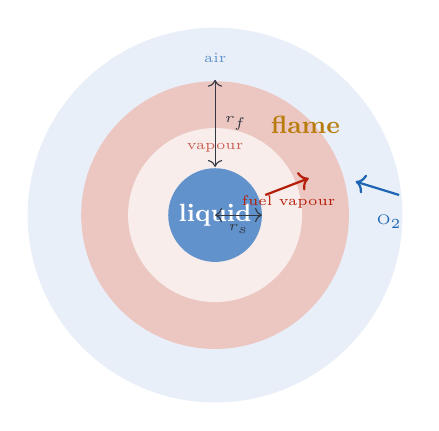
\begin{tikzpicture}[scale=0.85]
        % Ambient
        \fill[skyblue!10] (0,0) circle (2.8cm);
        % Flame surface
        \fill[firered!25] (0,0) circle (2.0cm);
        % Vapour zone
        \fill[firered!8] (0,0) circle (1.3cm);
        % Liquid droplet
        \fill[skyblue!70] (0,0) circle (0.7cm);
        % Labels
        \node[white,font=\small\bfseries] at (0,0) {liquid};
        \node[firered!70,font=\tiny] at (0,1.0) {vapour};
        \node[flameyellow!80!black,font=\small\bfseries] at (1.35,1.35)
          {flame};
        \node[skyblue!70,font=\tiny] at (0,2.35) {air};
        % Radii
        \draw[<->,ashgrey,thin] (0,0) -- (0.7,0)
          node[midway,below,font=\tiny]{$\rs$};
        \draw[<->,ashgrey,thin] (0,0.72) -- (0,2.02)
          node[midway,right,font=\tiny]{$r_f$};
        % Species arrows
        \draw[->,firered,thick] (0.75,0.3) -- (1.4,0.55);
        \node[firered,font=\tiny] at (1.1,0.2) {fuel vapour};
        \draw[->,skyblue,thick] (2.75,0.3) -- (2.1,0.5);
        \node[skyblue,font=\tiny] at (2.6,-0.1) {O$_2$};
      \end{tikzpicture}
    \end{column}
    \begin{column}{0.52\textwidth}
      Three concentric zones:
      \begin{enumerate}
        \item \textbf{Liquid droplet} ($r < \rs$):
              liquid fuel at $\Ts$ (wet-bulb)
        \item \textbf{Vapour zone} ($\rs < r < \rf$):
              fuel vapour diffuses outward;
              $Y_F > 0$, $Y_{\text{ox}} = 0$
        \item \textbf{Oxidiser zone} ($r > \rf$):
              air diffuses inward;
              $Y_F = 0$, $Y_{\text{ox}} > 0$
      \end{enumerate}
      \vspace{4pt}
      The \textbf{flame sheet} at $r = \rf$:
      \begin{itemize}
        \item All heat generated here
        \item Temperature peaks at $T_f \approx \Tad$
        \item $Y_F = Y_{\text{ox}} = 0$ simultaneously
              (Burke--Schumann limit)
      \end{itemize}
    \end{column}
  \end{columns}
\end{frame}

\begin{frame}{Burning Rate Constant and Flame Standoff Ratio}

  For a burning droplet, the evaporation rate is enhanced because
  the flame heats the surface.
  The mass burning rate is still:
  \[
    \mdot = 4\pi\rs\,\rho D\,\ln(1+\Bc)
  \]
  but with the \alert{combustion transfer number}:
  \[
    \Bc = \frac{Y_{\text{ox},\infty}/\nu + c_p(\Tinf - \Ts)/Q_{\text{HV}}}
              {1 + c_p(\Tinf - \Ts)/(Q_{\text{HV}}\,Y_{\text{ox},\infty}/\nu)}
    \approx \frac{Q_{\text{HV}}\,Y_{\text{ox},\infty}/(\nu c_p) + (\Tinf - \Ts)}
                 {L_v/c_p}
  \]
  where $\nu$ is the mass stoichiometric coefficient.

  \begin{block}{Burning rate constant $\Kc$}
    \[
      \Kc = \frac{8\rho D}{\rho_\ell}\ln(1+\Bc)
      \quad [\text{m}^2/\text{s}]
    \]
    Same form as $\Kd$ but with $\Bc \gg \BM$
    (combustion $\Rightarrow$ much faster evaporation).
    Typical ratio: $\Kc / \Kd \approx 3$--$10$.
  \end{block}

  \vspace{2pt}
  The \textbf{flame standoff ratio}:
  \[
    \frac{\rf}{\rs} = (1 + \nu\,Y_{\text{ox},\infty})^{1/3}
    \cdot \frac{1}{\Zst^{1/3}}
    \approx \left(\frac{\ln(1+\Bc)}{\ln(1+1/\Zst)}\right)^{1/3}
    \sim 3\text{--}6
  \]
\end{frame}

\begin{frame}{Radial Profiles in a Burning Droplet}

  \begin{center}
  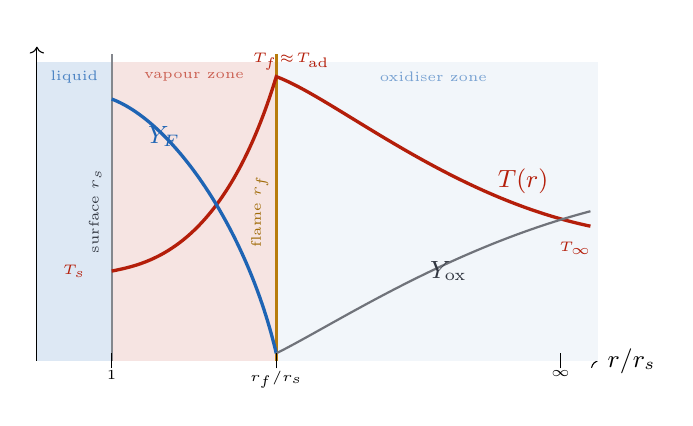
\begin{tikzpicture}[scale=0.95]
    % Axes
    \draw[->] (0,0) -- (7.5,0) node[right,font=\small]{$r/r_s$};
    \draw[->] (0,0) -- (0,4.2) node[above,font=\small]{};

    % Zone shading
    \fill[skyblue!15] (0,0) rectangle (1.0,4.0);
    \fill[firered!12] (1.0,0) rectangle (3.2,4.0);
    \fill[skyblue!6]  (3.2,0) rectangle (7.5,4.0);

    % Zone labels
    \node[skyblue!80,font=\tiny] at (0.5,3.8) {liquid};
    \node[firered!70,font=\tiny] at (2.1,3.8) {vapour zone};
    \node[skyblue!60,font=\tiny] at (5.3,3.8) {oxidiser zone};

    % Flame surface vertical line
    \draw[flameyellow!80!black,very thick] (3.2,0)--(3.2,4.1);
    \node[flameyellow!70!black,font=\tiny,rotate=90] at (2.98,2.0)
      {flame $r_f$};

    % Droplet surface
    \draw[ashgrey!60,thick] (1.0,0)--(1.0,4.1);
    \node[ashgrey,font=\tiny,rotate=90] at (0.78,2.0){surface $r_s$};

    % T profile: rises from Ts at surface, peaks at flame, decays to Tinf
    \draw[firered,very thick]
      (1.0,1.2)  % Ts at surface
      .. controls (1.5,1.3) and (2.5,1.5) ..
      (3.2,3.8)  % T_f at flame
      .. controls (4.0,3.5) and (5.5,2.2) ..
      (7.4,1.8); % Tinf far field
    \node[firered,font=\small] at (6.5,2.4){$T(r)$};
    \node[firered,font=\tiny] at (0.5,1.2){$T_s$};
    \node[firered,font=\tiny] at (3.4,4.0){$T_f \!\approx\! T_{\text{ad}}$};
    \node[firered,font=\tiny] at (7.2,1.5){$T_\infty$};

    % Y_F: high at surface, zero at flame
    \draw[skyblue,very thick]
      (1.0,3.5)  % Y_F,s at surface
      .. controls (1.8,3.2) and (2.8,1.8) ..
      (3.2,0.1); % zero at flame
    \node[skyblue,font=\small] at (1.7,3.0){$Y_F$};

    % Y_ox: zero at flame, rises to Y_ox,inf
    \draw[ashgrey!70,thick]
      (3.2,0.1)  % zero at flame
      .. controls (4.0,0.5) and (5.5,1.5) ..
      (7.4,2.0); % Y_ox,inf
    \node[ashgrey,font=\small] at (5.5,1.2){$Y_{\text{ox}}$};

    % x-axis ticks
    \draw (1.0,-0.1)--(1.0,0.1); \node[below,font=\tiny] at (1.0,0){1};
    \draw (3.2,-0.1)--(3.2,0.1); \node[below,font=\tiny] at (3.2,0){$r_f/r_s$};
    \draw (7.0,-0.1)--(7.0,0.1); \node[below,font=\tiny] at (7.0,0){$\infty$};
  \end{tikzpicture}
  \end{center}

  \small Temperature peaks at the flame sheet; fuel and oxidiser
  profiles meet at zero simultaneously (Burke--Schumann).
\end{frame}

\begin{frame}{Droplet Lifetime: Combustion vs.\ Pure Evaporation}

  \begin{columns}[t]
    \begin{column}{0.50\textwidth}
      \textbf{Droplet lifetime}
      \[
        \td = \frac{D_0^2}{\Kc}
        = \frac{\rho_\ell D_0^2}{8\rho D\ln(1+\Bc)}
      \]

      For Jet-A at $T_\infty = 1500$ K, $p = 10$ bar:
      \begin{center}
      \renewcommand{\arraystretch}{1.2}
      \begin{tabular}{lcc}
        \toprule
        $D_0\,(\mu\text{m})$ & $\td$ (ms) \\
        \midrule
        30  & 0.14 \\
        50  & 0.39 \\
        100 & 1.56 \\
        200 & 6.25 \\
        \bottomrule
      \end{tabular}
      \end{center}

      Gas turbine requirement: complete burnout in
      $\sim$3--8 ms $\Rightarrow$ \alert{$D_0 < 80\,\mu$m}
      essential.
    \end{column}
    \begin{column}{0.46\textwidth}
      \textbf{Effect of $\Bc$ vs.\ $\BM$}
      \begin{itemize}
        \item Without combustion: $\Kd \sim 10^{-7}$ m$^2$/s
              (pure evaporation in hot air)
        \item With combustion: $\Kc \sim 5\times10^{-7}$ m$^2$/s
              (flame heats surface strongly)
        \item Ratio $\Kc/\Kd = \ln(1+\Bc)/\ln(1+\BM)$;
              typically 3--6$\times$ faster burning
              than pure evaporation
      \end{itemize}

      \begin{alertblock}{Atomisation design rule}
        $\td \propto D_0^2$: halving droplet diameter
        reduces lifetime by \textbf{4}$\times$.
        Finer atomisation is the most powerful lever
        for combustor efficiency.
      \end{alertblock}
    \end{column}
  \end{columns}
\end{frame}

% =====================================================================
\section{Corrections to the D\texorpdfstring{$^2$}{2} Law}
% =====================================================================

\begin{frame}{Forced Convection: Ranz--Marshall Correction}

  The D$^2$ law assumes a \textbf{quiescent} environment.
  In practice, droplets move relative to the gas (slip velocity $u_s$),
  increasing heat and mass transfer.

  \begin{block}{Ranz--Marshall correlation}
    \[
      \Sh = 2 + 0.6\,\Rey_d^{1/2}\,\Sc^{1/3}
      \qquad
      \Nu = 2 + 0.6\,\Rey_d^{1/2}\,\Pr^{1/3}
    \]
    where $\Rey_d = u_s D/\nu$ is the droplet Reynolds number.
    The corrected evaporation rate:
    \[
      \mdot_{\text{conv}} = \pi D\,\rho D_{\text{AB}}\,\Sh\,
                            \ln(1+\BM)
    \]
  \end{block}

  \begin{columns}[t]
    \begin{column}{0.50\textwidth}
      \textbf{Practical effect}
      \begin{itemize}
        \item $\Rey_d \sim 10$--$50$ in gas turbine sprays
        \item $\Sh \approx 3$--$5$ (vs.\ $\Sh = 2$ at rest)
        \item Evaporation rate increased by $\Sh/2 \approx 1.5$--$2.5\times$
        \item Lifetime reduced accordingly
      \end{itemize}
    \end{column}
    \begin{column}{0.46\textwidth}
      \textbf{Modified D$^2$ law (corrected)}
      \[
        \frac{d(D^2)}{dt} = -\Kd\cdot\frac{\Sh}{2}
      \]
      For $\Rey_d \ll 1$ (Stokes flow): $\Sh \to 2$, recovers
      original D$^2$ law.
    \end{column}
  \end{columns}
\end{frame}

\begin{frame}{Other Corrections}

  \begin{columns}[t]
    \begin{column}{0.50\textwidth}
      \textbf{Variable properties}\\[3pt]
      Use the ``1/3 rule'' reference temperature:
      \[
        T_{\text{ref}} = \Ts + \tfrac{1}{3}(\Tinf - \Ts)
      \]
      Evaluate $\rho$, $\mu$, $D$, $\lambda$ at $T_{\text{ref}}$.
      This accounts for the large temperature gradient across the
      vapour film without iterative property evaluation.

      \vspace{6pt}
      \textbf{Internal circulation}\\[3pt]
      Real droplets have internal liquid-phase recirculation
      (Hill vortex) that accelerates heat conduction inside the
      droplet and reduces the heat-up time.
      Effect: $\td$ can be 10--20\% shorter than D$^2$ prediction.
    \end{column}
    \begin{column}{0.46\textwidth}
      \textbf{Multi-component fuel}\\[3pt]
      Jet-A contains $\sim$200 hydrocarbon species spanning
      a wide volatility range.
      \begin{itemize}
        \item Light fractions evaporate first
        \item Droplet composition drifts toward heavier components
        \item $\Yfs$ decreases as $\Ts$ is limited by
              higher-boiling species
        \item Distillation curve models replace
              single-component assumption
      \end{itemize}

      \vspace{4pt}
      \textbf{High-pressure effects}\\[3pt]
      At $p > p_c$ (critical pressure), the liquid--vapour
      interface vanishes.
      Transcritical injection: no surface tension, no distinct
      droplet; classical D$^2$ law breaks down.
    \end{column}
  \end{columns}
\end{frame}

\begin{frame}{Pressure Dependence of $\Kc$}

  From the burning rate expression
  $\Kc = 8\rho D\ln(1+\Bc)/\rho_\ell$:
  \begin{itemize}
    \item $\rho D \approx \text{const}$ at fixed temperature
          (kinetic theory: $D \propto 1/p$, $\rho \propto p$)
    \item $\rho_\ell$ is nearly pressure-independent (liquid)
    \item $\Bc$ depends on $\Yfs(p, \Ts)$ and $Q_{\text{HV}}/c_p$;
          weakly pressure-dependent
  \end{itemize}

  \begin{block}{Key result}
    \[
      \Kc \approx \text{const} \text{ w.r.t.\ } p
      \quad\Rightarrow\quad
      \td = \frac{D_0^2}{\Kc} \approx \text{const}
    \]
    Droplet lifetime is \textbf{approximately pressure-independent}
    for classical evaporation-controlled burning.
    This is a striking contrast to premixed flame speed
    ($S_L \propto p^{-0.13}$) and is one reason liquid-fuel
    combustors can operate over a wide pressure range.
  \end{block}

  \begin{alertblock}{Caveat}
    Near the critical pressure, $\Bc$ and $\Yfs$ change rapidly
    and $\td$ can decrease significantly.
    Rocket chambers at $> 50$ bar enter this regime.
  \end{alertblock}
\end{frame}

% =====================================================================
\section{Ignition and Extinction of Burning Droplets}
% =====================================================================

\begin{frame}{Droplet Ignition}

  For a burning droplet to form, the vapour--air mixture
  surrounding the droplet must be ignited.

  \begin{columns}[t]
    \begin{column}{0.50\textwidth}
      \textbf{Critical conditions for ignition}
      \begin{itemize}
        \item The ambient temperature must exceed the
              \textbf{auto-ignition temperature} of the vapor--air
              mixture at the droplet surface
        \item Or an external ignition source (spark, hot surface,
              pilot flame) must provide the activation energy
        \item After ignition, the flame quickly wraps around the
              droplet to form the spherical shell geometry
        \item Ignition delay $t_{\text{ign}}$ must be shorter than
              the droplet lifetime $\td$
      \end{itemize}
    \end{column}
    \begin{column}{0.46\textwidth}
      \textbf{Ignition criterion}
      \[
        t_{\text{ign}} < \td
        \quad\Rightarrow\quad
        \frac{D_0^2 / \Kd}{\tchem(T_\infty)}
        = \Da_{\text{droplet}} > 1
      \]
      At low ambient temperature or high velocity:
      \begin{itemize}
        \item Droplet evaporates and cools the surrounding gas
        \item Mixture never reaches auto-ignition
        \item Result: evaporation without combustion
              (``wet'' spray)
      \end{itemize}

      \begin{exampleblock}{Gas turbine relight}
        At altitude, low $T_3$ and high droplet Reynolds number
        can prevent ignition --- the spark must heat a sufficient
        volume of vapor--air to overcome this.
      \end{exampleblock}
    \end{column}
  \end{columns}
\end{frame}

\begin{frame}{Droplet Extinction}

  A burning droplet extinguishes when the flame can no longer
  sustain itself.  The extinction criterion mirrors the WSR
  blowout condition (Unit 4):

  \[
    \Da_{\text{flame}} = \frac{t_{\text{residence,flame}}}{\tchem}
    = \frac{(r_f - r_s)^2 / \alpha}{\tchem} < \Da_{\text{crit}} \approx 1
  \]

  \begin{itemize}
    \item As $D \to 0$: $\rf \to 0$, flame zone shrinks, residence
          time decreases, $\Da \to 0$, extinction inevitable
    \item There exists a \textbf{critical diameter} $D_{\text{ext}}$
          below which no flame can be sustained:
          \[
            D_{\text{ext}} \sim \frac{\alpha}{\Kc^{1/2}} \cdot f(\Bc)
            \quad\sim 10\text{--}50\,\mu\text{m}
          \]
    \item Droplets smaller than $D_{\text{ext}}$ evaporate without
          burning --- their vapor mixes with the surrounding gas
          and burns in the bulk flame
    \item Important for spray combustion modeling: not all
          droplets burn as isolated spheres
  \end{itemize}
\end{frame}

% =====================================================================
\section{Spray Combustion and Aero Applications}
% =====================================================================

\begin{frame}{From Single Droplet to Spray Combustion}

  Real combustors contain $\sim 10^6$--$10^9$ droplets per
  cubic metre.
  Spray combustion is characterized by the interaction between
  droplets and their surroundings.

  \begin{columns}[t]
    \begin{column}{0.52\textwidth}
      \textbf{Key spray parameters}
      \begin{itemize}
        \item \textbf{Sauter Mean Diameter (SMD)} $D_{32}$:
              droplet diameter with the same volume/surface ratio
              as the spray distribution --- the D$^2$ law lifetime
              is estimated using $D_{32}$
        \item \textbf{Droplet number density} $n$: affects inter-
              droplet interactions (group combustion)
        \item \textbf{Stokes number} $\mathrm{St} = \tau_d/\tau_f$:
              ratio of droplet relaxation time to flow time;
              controls whether droplets follow the gas ($\mathrm{St} \ll 1$)
              or not ($\mathrm{St} \gg 1$)
      \end{itemize}
    \end{column}
    \begin{column}{0.44\textwidth}
      \textbf{Group combustion number}
      \[
        G = n^{1/3} D_0 \cdot \frac{\rf}{D_0}
      \]
      \begin{itemize}
        \item $G \ll 1$: isolated droplet combustion
        \item $G \sim 1$: internal group combustion
        \item $G \gg 1$: external group combustion
              (spray surrounded by one large flame)
      \end{itemize}
      \small Gas turbine sprays typically span
      $G \sim 0.1$--$10$ depending on the
      local drop density.
    \end{column}
  \end{columns}
\end{frame}

\begin{frame}{Gas Turbine Combustor: Droplet Lifetime Budget}

  \begin{center}
  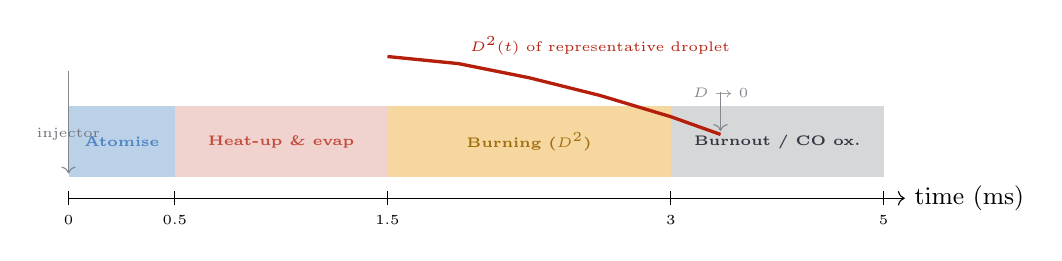
\begin{tikzpicture}[font=\small, scale=0.9]
    % Timeline bar
    \fill[ashgrey!15] (0,-0.5) rectangle (11.5,0.5);
    % Phases
    \fill[skyblue!30]   (0,-0.5)   rectangle (1.5,0.5); % atomisation
    \fill[firered!20]   (1.5,-0.5) rectangle (4.5,0.5); % heat-up / evap
    \fill[flameyellow!40](4.5,-0.5) rectangle (8.5,0.5); % combustion
    \fill[ashgrey!20]   (8.5,-0.5) rectangle (11.5,0.5); % burnout
    % Labels inside bar
    \node[font=\tiny\bfseries,skyblue!80]   at (0.75,0)  {Atomise};
    \node[font=\tiny\bfseries,firered!80]   at (3.0,0)   {Heat-up \& evap};
    \node[font=\tiny\bfseries,flameyellow!70!black] at (6.5,0)  {Burning ($D^2$)};
    \node[font=\tiny\bfseries,ashgrey]      at (10.0,0)  {Burnout / CO ox.};
    % Time axis
    \draw[->] (0,-0.8) -- (11.8,-0.8)
      node[right,font=\small]{time (ms)};
    \foreach \t/\lab in {0/0, 1.5/0.5, 4.5/1.5, 8.5/3, 11.5/5}{
      \draw (\t,-0.7)--(\t,-0.9);
      \node[below,font=\tiny] at (\t,-0.9){\lab};
    }
    % D^2 curve above bar
    \draw[firered,very thick]
      (4.5,1.2) -- (5.5,1.1) -- (6.5,0.9)
      -- (7.5,0.65) -- (8.5,0.35) -- (9.2,0.1);
    \node[firered,font=\tiny] at (7.5,1.35) {$D^2(t)$ of representative droplet};
    % Arrows
    \draw[->,ashgrey!60,thin] (0,1.0)--(0,-0.45)
      node[above,font=\tiny,ashgrey!70,yshift=0.3cm]{injector};
    \draw[->,ashgrey!60,thin] (9.2,0.7)--(9.2,0.15)
      node[above,font=\tiny,yshift=0.3cm]{$D\to 0$};
  \end{tikzpicture}
  \end{center}

  \vspace{0.1cm}
  \begin{itemize}
    \item Atomization: pressure-swirl nozzle creates SMD
          $\sim$ 30--80 $\mu$m in $< 0.5$ ms
    \item Heat-up + evaporation: $\sim$ 1 ms; governed by $\BM$
    \item Burning: D$^2$ law applies; $\td \sim 1$--$3$ ms for
          $D_{32} = 50$--$80\,\mu$m
    \item Burnout: CO oxidation in the lean zone (WSR + PFR,
          Units 4--5)
  \end{itemize}
\end{frame}

\begin{frame}{Rocket Combustion: Extreme Droplet Conditions}

  \begin{columns}[t]
    \begin{column}{0.52\textwidth}
      \textbf{LOX/kerosene (RD-180 type)}
      \begin{itemize}
        \item $p_c = 250$ bar --- supercritical for oxygen
              ($p_c^{\text{O}_2} = 50$ bar)
        \item No classical droplet: trans-critical injection
              creates ``dense fluid'' jets, not spray
        \item D$^2$ law inapplicable; supercritical mixing models
              used instead
        \item $T_c \approx 3500$ K; $\rho_c \approx 120$ kg/m$^3$
      \end{itemize}

      \vspace{4pt}
      \textbf{LOX/LH$_2$ (Vulcain 2 type)}
      \begin{itemize}
        \item $p_c = 110$ bar --- also supercritical for both
              propellants
        \item Coaxial shear-layer combustion
        \item Flame length $\sim$ 10--30 mm per element
      \end{itemize}
    \end{column}
    \begin{column}{0.44\textwidth}
      \textbf{Subcritical case: RP-1/LOX at moderate $p$}
      \begin{itemize}
        \item D$^2$ law with corrections applicable
        \item $\Bc \sim 5$--$8$ (very volatile in hot $O_2$)
        \item $\Kc \sim 3\times10^{-6}$ m$^2$/s
        \item $D_{32} \sim 100\,\mu$m $\Rightarrow$
              $\td \sim 3\,\mu$s (!!)
        \item Must complete combustion in $< 10$--$20$ ms
              (chamber stay time)
      \end{itemize}

      \begin{exampleblock}{Design constraint}
        Chamber length set by
        $L^* = V_c / A_t \sim 0.5$--$1.0$ m for RP-1/LOX,
        where $A_t$ is throat area.
        Droplet lifetime budget drives this.
      \end{exampleblock}
    \end{column}
  \end{columns}
\end{frame}

% =====================================================================
\section{Summary}
% =====================================================================

\begin{frame}{Key Equations at a Glance}
  \renewcommand{\arraystretch}{1.6}
  \begin{tabular}{>{\bfseries}p{3.8cm} p{8.0cm}}
    \toprule
    Concept & Expression \\
    \midrule
    D$^2$ law & $D^2(t) = D_0^2 - Kt$; \quad $t_d = D_0^2/K$ \\
    Evaporation constant & $K = 8\rho D\ln(1+B_M)/\rho_\ell$ \\
    Mass transfer number & $B_M = (Y_{F,s} - Y_{F,\infty})/(1-Y_{F,s})$ \\
    Thermal transfer number & $B_T \approx c_p(T_\infty-T_s)/L_v$ \\
    Combustion transfer no. & $B_c \approx Q_{\text{HV}} Y_{\text{ox},\infty}/(\nu c_p L_v/c_p)$ \\
    Burning rate constant & $K_c = 8\rho D\ln(1+B_c)/\rho_\ell$ \\
    Flame standoff ratio & $r_f/r_s \approx [\ln(1+B_c)/\ln(1+1/Z_{\text{st}})]^{1/3}$ \\
    Ranz--Marshall & $\mathrm{Sh} = 2 + 0.6\,\mathrm{Re}_d^{1/2}\,\mathrm{Sc}^{1/3}$ \\
    \bottomrule
  \end{tabular}
\end{frame}

\begin{frame}{Summary \& Take-Away Points}
  \begin{itemize}
    \item The \textbf{D$^2$ law}: droplet diameter squared decreases
          linearly with time; lifetime $t_d = D_0^2/K$.
          This is the single most important result in droplet combustion.
    \item The \textbf{Spalding transfer number} $B_M$ (or $B_c$)
          encapsulates all thermochemical driving forces for
          evaporation or burning into one dimensionless parameter.
    \item A \textbf{spherical diffusion flame} forms at the
          stoichiometric surface $r = r_f \approx 3$--$6\,r_s$;
          the flame greatly enhances the evaporation rate
          ($K_c \approx 3$--$10 \times K_d$).
    \item \textbf{Droplet lifetime} $t_d \propto D_0^2$: finer
          atomization is the most powerful lever for combustor
          efficiency and compactness.
    \item The D$^2$ law assumes quiescent surroundings; forced
          convection (Ranz--Marshall) increases evaporation by
          $\mathrm{Sh}/2 \approx 2$--$3\times$.
    \item At \textbf{high pressure} ($p > p_c$), classical D$^2$
          theory breaks down; supercritical mixing models are required
          (relevant for liquid rocket engines).
  \end{itemize}
  \vfill
  \begin{center}
    \large\textbf{Next lecture:} Spray Atomization and Droplet Size
    Distributions
  \end{center}
\end{frame}

% -- Closing slide ----------------------------------------------------
{
\setbeamertemplate{footline}{}
\setbeamertemplate{headline}{}
\setbeamercolor{background canvas}{bg=ashgrey}
\begin{frame}[plain, c]

  \begin{tikzpicture}[remember picture, overlay]
    \fill[ashgrey]
      (current page.south west) rectangle (current page.north east);
    \fill[firered, opacity=0.15]
      (current page.south east) circle (4.5cm);
    \fill[flameyellow, opacity=0.08]
      (current page.south east) circle (2.5cm);
  \end{tikzpicture}

  \vspace{0.55cm}
  {\color{white}\fontsize{22}{26}\selectfont\bfseries
   Droplet Evaporation and Combustion}

  \vspace{0.10cm}
  {\color{skyblue!70}\fontsize{9}{11}\selectfont
   Unit 8\enspace|\enspace
   Propulsion \& Combustion\enspace|\enspace
   Aeronautical Engineering Yr\,4}

  \vspace{0.12cm}
  
\begin{tikzpicture}
    \draw[skyblue!60, line width=0.6pt] (0,0) -- (\textwidth,0);
    \draw[firered,    line width=2.2pt] (0,0) -- (0.28\textwidth,0);
  \end{tikzpicture}

  \vspace{0.30cm}

  \begin{columns}[t, totalwidth=\textwidth]
    \begin{column}{0.315\textwidth}
      \begin{beamercolorbox}[rounded=true,wd=\linewidth,
                             sep=6pt,center]{block title}
        \textbf{\small D$^2$ Law \& Transfer Numbers}
      \end{beamercolorbox}
      \vspace{3pt}
      \begin{beamercolorbox}[rounded=true,wd=\linewidth,
                             sep=6pt,center]{block body}
        \color{ashgrey}\fontsize{7.5}{10}\selectfont
        $D^2(t) = D_0^2 - Kt$\\[3pt]
        Spalding $B_M$, $B_T$, $B_c$\\[3pt]
        Wet-bulb temperature\\[3pt]
        $t_d \propto D_0^2$: atomisation lever
      \end{beamercolorbox}
    \end{column}
    \hfill
    \begin{column}{0.315\textwidth}
      \begin{beamercolorbox}[rounded=true,wd=\linewidth,
                             sep=6pt,center]{block title alerted}
        \textbf{\small Single Droplet Flame}
      \end{beamercolorbox}
      \vspace{3pt}
      \begin{beamercolorbox}[rounded=true,wd=\linewidth,
                             sep=6pt,center]{block body alerted}
        \color{ashgrey}\fontsize{7.5}{10}\selectfont
        Spherical diffusion flame at $r_f$\\[3pt]
        Standoff ratio $r_f/r_s \approx 3$--$6$\\[3pt]
        $K_c \approx 3$--$10\times K_d$\\[3pt]
        Extinction at $D < D_{\text{ext}}$
      \end{beamercolorbox}
    \end{column}
    \hfill
    \begin{column}{0.315\textwidth}
      \begin{beamercolorbox}[rounded=true,wd=\linewidth,
                             sep=6pt,center]{block title example}
        \textbf{\small Propulsion Context}
      \end{beamercolorbox}
      \vspace{3pt}
      \begin{beamercolorbox}[rounded=true,wd=\linewidth,
                             sep=6pt,center]{block body example}
        \color{white}\fontsize{7.5}{10}\selectfont
        GTE: SMD $< 80\,\mu$m for burnout\\[3pt]
        Ranz--Marshall: forced convection\\[3pt]
        Rocket: supercritical ($p > p_c$)\\[3pt]
        $t_d \approx$ const w.r.t.\ $p$
      \end{beamercolorbox}
    \end{column}
  \end{columns}

  \vspace{0.30cm}

  \begin{beamercolorbox}[rounded=true,wd=\textwidth,
                         sep=5pt,center]{block body}
    \color{skyblue!80}\fontsize{7.8}{10}\selectfont
    $D^2 = D_0^2 - Kt$
    \quad\vrule width 0.4pt height 9pt depth 2pt\quad
    $K = 8\rho D\ln(1+B)/\rho_\ell$
    \quad\vrule width 0.4pt height 9pt depth 2pt\quad
    $t_d = D_0^2/K$
    \quad\vrule width 0.4pt height 9pt depth 2pt\quad
    $\mathrm{Sh} = 2 + 0.6\,\mathrm{Re}_d^{1/2}\,\mathrm{Sc}^{1/3}$
  \end{beamercolorbox}

  \vspace{0.22cm}
  \begin{center}
    {\color{white!50}\fontsize{7.5}{9}\selectfont
     \textbf{Next:}\enspace
     Turbulent Combustion}
  \end{center}
\end{frame}
}

% =====================================================================
\appendix
\begin{frame}{Practice Problems}
  \begin{enumerate}
    \item A Jet-A droplet ($D_0 = 60\,\mu$m, $\rho_\ell = 800$ kg/m$^3$)
          evaporates in hot air at $T_\infty = 1200$ K, $p = 10$ bar.
          Given $\rho D = 5\times10^{-5}$ kg/(m$\cdot$s) and
          $B_M = 1.5$, calculate the evaporation constant $K$ and the
          droplet lifetime $t_d$.
          If the droplet is burning ($B_c = 4.5$), how does $t_d$
          change?

    \item Derive the D$^2$ law from first principles starting from the
          spherically symmetric mass conservation equation.
          State clearly which assumptions are invoked at each step and
          identify the physical meaning of the Spalding number $B_M$.

    \item For a burning Jet-A droplet at 1 atm and $T_\infty = 1500$ K,
          the flame standoff ratio is $r_f/r_s = 4$.
          Sketch the radial profiles of $T(r)$, $Y_F(r)$, and
          $Y_{\text{ox}}(r)$, labeling all key values.
          Explain why $T$ at the droplet surface is lower than $T_\infty$.

    \item A gas turbine combustor has a residence time of 5 ms.
          Using the D$^2$ law with $K_c = 4\times10^{-7}$ m$^2$/s,
          determine the \emph{maximum} initial droplet diameter $D_0$
          that ensures complete evaporation before the gas exits the
          primary zone.
          Comment on the role of the Ranz--Marshall correction.
  \end{enumerate}
\end{frame}

\end{document}
